\subsection{Test di significatività globale}

Una prima verifica d'ipotesi che si può fare è quella sull'ipotesi che il modello lineare non serva per spiegare la relazione con l'alternativa, la quale dice che almeno a qualcosa serve.

$$
\begin{cases}
H_0 : \beta_1 = \beta_2 = \ldots = \beta_p = 0 \\
H_1 : \text{almeno un }\beta_j \neq 0 \quad j = 1 \ldots p
\end{cases}
$$

la verifica dell'ipotesi si fa al solito modo, utilizzando $ F_{oss} $ che dipende da $ R^2 $:

\begin{align*}
F_{oss} &= \frac{R^2}{1-R^2} \frac{n - p}{p} \\
			 &= \frac{\text{devianza spiegata}}{\text{devianza residua}} \cdot \frac{n - p}{p-1} \\
			 &= \frac{\sum_{i=1}^{n} (\hat{y}_i - \bar{y})^2}{\sum_{i=1}^{n} (y_i - \hat{y}_i)^2} \cdot \frac{n - p}{p -1} \\
			 &= \frac{\sum_{i=1}^{n} (\hat{y}_i - \bar{y})^2 \big/ (p-1)}{\sum_{i=1}^{n} (y_i - \hat{y}_i)^2 \big/(n-p)}
\end{align*}

\subsubsection{Riassumendo}

Con la notazione $ MSR $ ci si riferisce alla somma dei quadrati degli scarti delle regressione ($ SSR $) divisi i gradi di libertà della regressione, ottenendo quindi:

$$
MRS = \frac{SSR}{p}
$$

In modo analogo 

$$
MST = \frac{SST}{n} \quad \text{e} \quad MSE = \frac{SSE}{n-p}
$$

ovvero $ MST $ coincide con la varianza totale.



\section{Gestione delle variabili esplicative}

\textbf{Dataset di riferimento} informazione sui distretti di Boston, si vuole far previsione sul costo medio della casa.

Tracciando i vari diagrammi di dispersione per le variabili esplicative del dataset è possibile notare se queste sono tra loro correlate.

Una volta notata una sorta di correlazione è possibile provare ad utilizzare tutte le variabili per calcolare il modello lineare:

$$
\text{(valore)} = \beta_0 + \beta_1 \text{(crimine)} + \ldots + \beta_13 \text{(poveri)} + \text{errore}
$$

C'è però da notare una cosa, il dataset contiene delle variabili qualitative, come \textit{fiume} che può prendere come valore \textit{0 o 1} e \textit{str} che ha 9 possibili valori.

Per poter utilizzare il modello lineare è necessario trasformare queste variabili discrete che possono assumere \textit{k} valori in $ k -1 $ variabili \textbf{indicatrici} o \textbf{dummies}, una per ogni possibile valore (meno uno), che possono assumere come valore \textit{0 o 1} e tali che al massimo una sola di queste variabili sia a 1.

Viene utilizzata una variabile in meno rispetto al numero dei valori perché il valore escluso (che viene fissato a priori) viene rappresentato quando tutte le altre variabili sono a 0.

La scelta del valore influisce sul significato dei parametri. Ovvero fissato un parametro di default (con tutte le variabili indicatrici a 0) i valore degli altri parametri esprire la variazione rispetto al parametro di default.

Ad esempio considerando reddito~regione. Se la regione di default è il Veneto, gli altri parametri associati alle variabili dummies indicando la variazione del reddito in base a quello del veneto: le regioni più povere avranno un parametro negativo, mentre quelle più ricche del veneto avranno un parametro positivo.

Tornando ad dataset delle case, si ottiene quindi una matrice $ \textbf{X} $ con 506 righe e 21 colonne.

\subsection{Verifica d'ipotesi per i coefficienti}

In modo simile a come avviene con il modello a due parametri è possibile formulare le ipotesi:

$$
\begin{cases}
H_0 : \beta_i = 0\\
H_1 : \beta_i \neq 0
\end{cases}
$$

che vengono verificate utilizzando

\begin{align*}
t_{oss}(\beta_i) &= \frac{\hat{\beta}_i}{\sqrt{\cfrac{s^2}{\sum_{j=1}^{n} (x_{ij} - \bar{x}_i)^2}}} = \frac{\hat{\beta}_i}{ \sqrt{\cfrac{ \sum_{j=1}^{n}(y_{ij} - \hat{y}_j)^2 /(n-p) }{ \sum_{j=1}^{n} (s_{ij} - \bar{x}_i)^2 } } } \\
&= \frac{\vec{a}^T \hat{\beta}}{ s \sqrt{\vec{a}^T (\textbf{X}^T\textbf{X} )^{-1} \vec{a}} }
\end{align*}

dove $ \vec{a} $ è un vettore con tanti elementi quanti sono i parametri, che contiene tutti 0 tranne nell'elemento $ i $-esimo.

La statistica $ t_{oss} $ sotto $ H_0 $ si distribuisce come una $ t $ di Student con $ n-p $ gradi di liberà.
Nel caso d'esempio si ha $ n - p = 506-21 = 485 $. Da notare che \textit{p} tiene conto anche di $ \beta_0 $

Da verificar che $ n - \#var -1 = n-p $.\\


\subsection{Adattamento complessivo del modello}

Come prima si può calcolare $ R^2 $ come

$$
R^2 = \frac{ \hat{\beta}^T \textbf{X}^T\vec{y} - n\bar{y}^2}{ \vec{y}^T\vec{y} - n\bar{y}^2 }
$$

La significatività di $R^2$ può essere valutata attraverso

\begin{align*}
F_{oss} &= \frac{\text{media dei quadrati degli scarti spiegati}}{\text{media dei quadrati degli scarti residui}}\\
			 &=  \frac{ \hat{\beta}^T \textbf{X}^T\vec{y} - n\bar{y}^2 /(p-1) }{ \vec{y}^T\vec{y} - n\bar{y}^2 /(n-p)}
\end{align*}
\todo{Nelle slide c'è n-1 al posto di p-1, solo nella formula}


Sotto $ H_0 $ $ F_{oss} $ si distribuisce come una $ F $ di Snedecor con $ p-1 $ gradi di libertà al numeratore e $ n-p $ gradi di libertà al denominatore

\subsection{Valutazione del primo modello}

\begin{figure}[htbp]
	\centering
	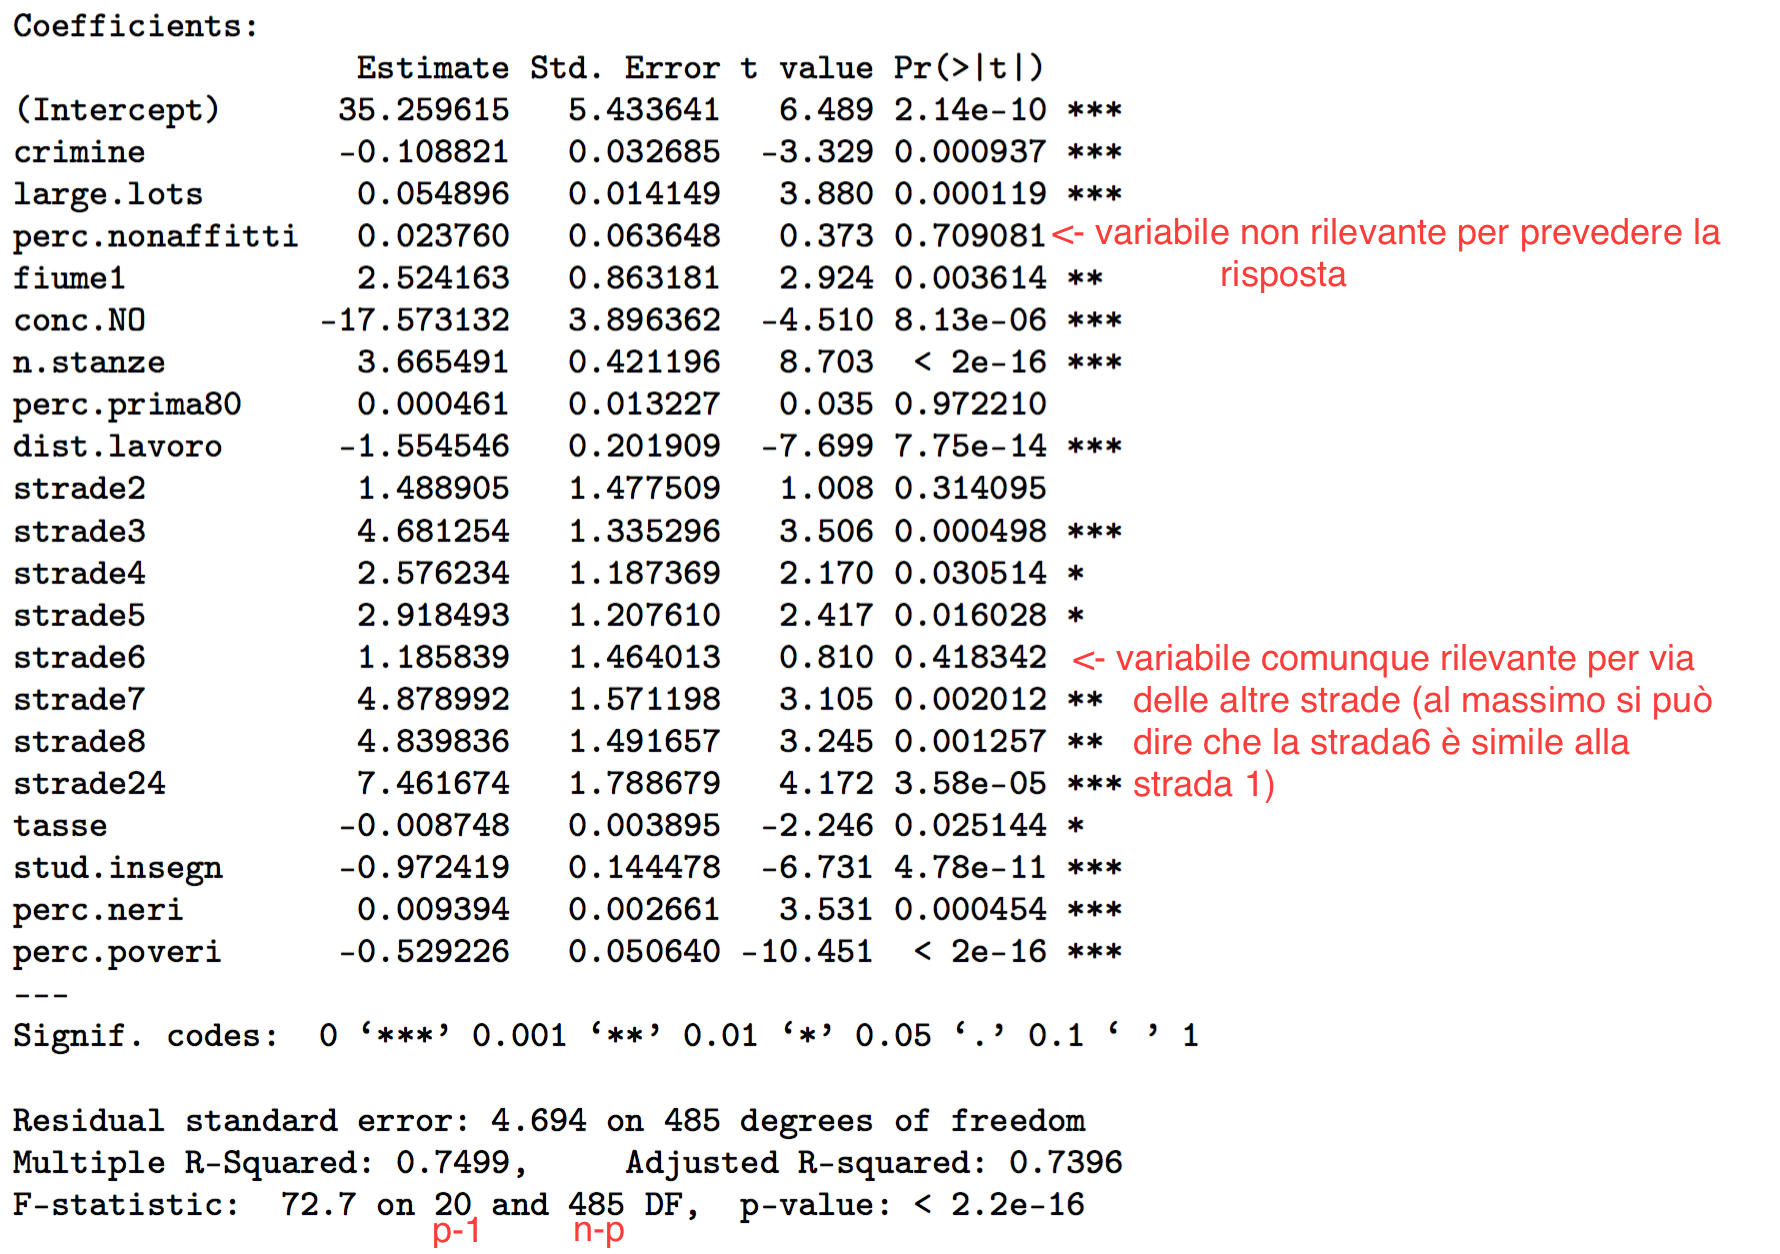
\includegraphics[width=.7\textwidth]{./notes/immagini/l10-fig1.png}
\end{figure}

\begin{figure}[htbp]
	\centering
	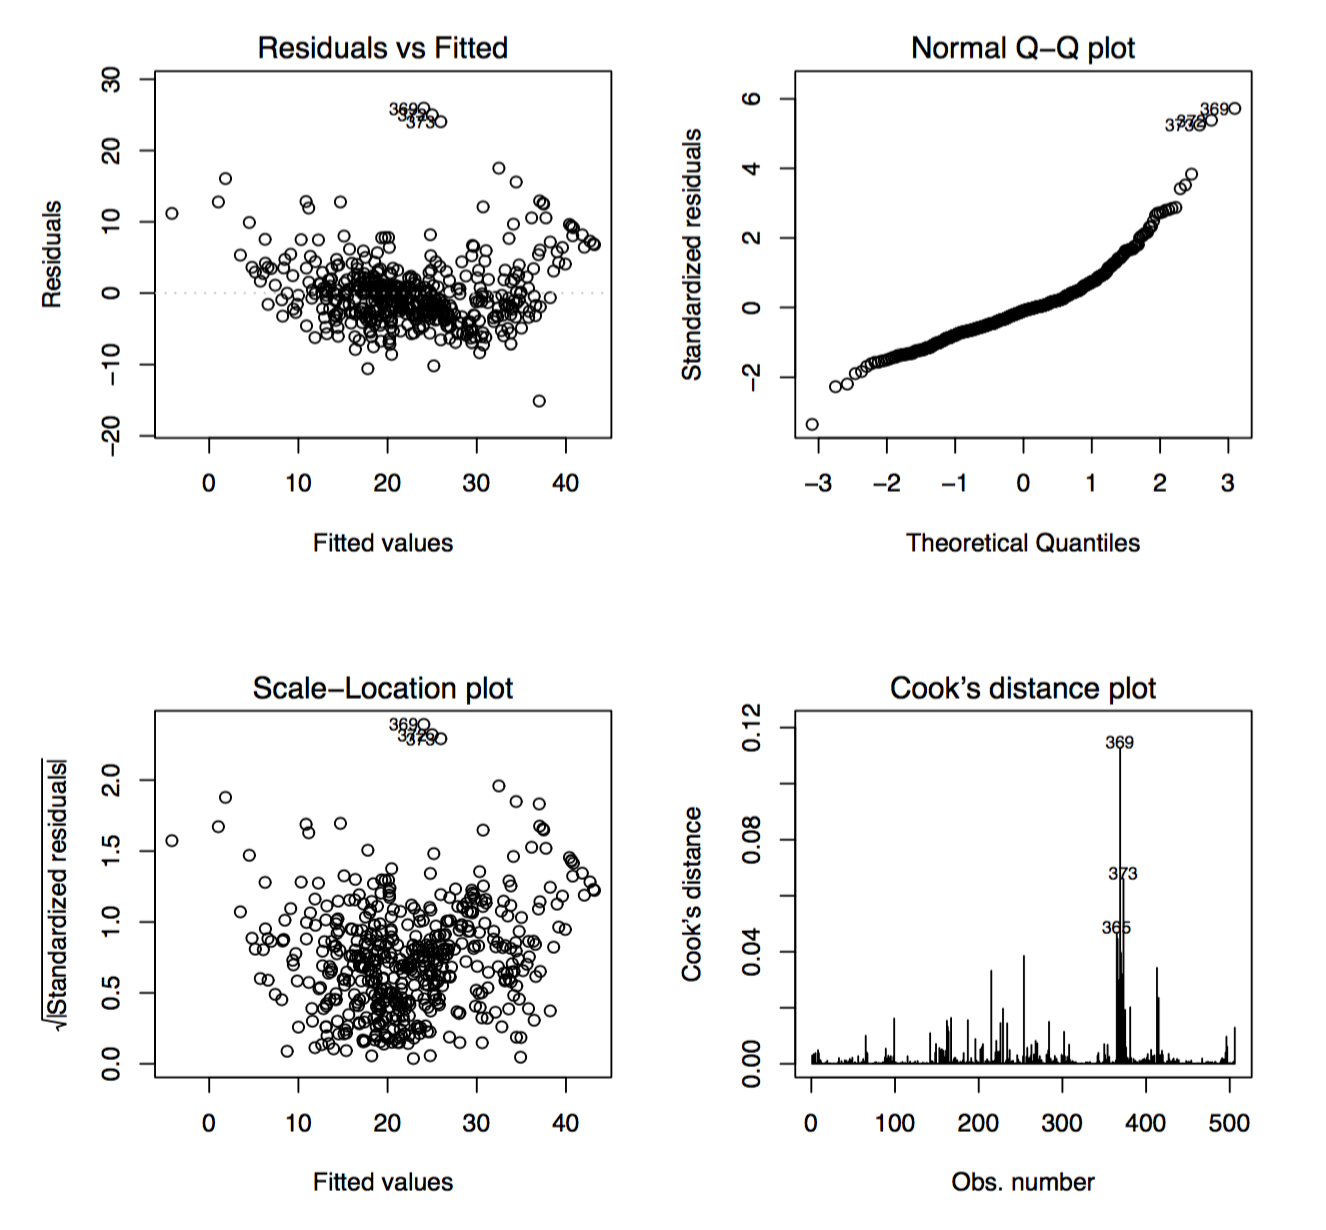
\includegraphics[width=.7\textwidth]{./notes/immagini/l10-fig2.png}
\end{figure}

Come si può notare il modello ottenuto risulta essere abbastanza buono, tuttavia:

\begin{itemize}
	\item Nel grafico dei residui si nota una forma ad U e la presenza di alcuni valori particolari
	\item Le code del QQ-Plot si allontanano dalla distribuzione normale
	\item Ci sono dei valori più significativi che influenzano il modello
\end{itemize}

Si può quindi provare ad applicare delle trasformazioni delle variabili e ad omettere i valori troppo influenti, in modo da ottenere un $ R^2 $ maggiore.

Da notare che in questo caso $ R^2 $ può essere confrontato con quello precedentemente ottenuto perché le trasformazioni non riguardano la variabile risposta.

\subsection{Analisi della varianza per la scelta delle variabili esplicative}

Avendo a disposizione tante variabili può essere che ce ne siano alcune di non significative per il modello.

Serve quindi un meccanismo formale per cercare e rimuovere queste variabili, tenendo conto che l'inclusione o l'esclusione di una singola variabile influisce sulla varianza dei residui. Questa procedura prende il nome di \textbf{analisi della varianza}.

Si è già visto come scomporre la varianza:

$$
\underbrace{\sum\limits_{i=1}^n (y_i - \bar{y})^2}_{\text{devianza}} = \underbrace{\sum\limits_{i=1}^n (\hat{y}_i - \bar{y})^2}_{\text{devianza spiegata dal modello}} + \underbrace{\sum\limits_{i=1}^n (y_i - \hat{y}_i)^2}_{\text{devianza residua}}  
$$

Nel caso della regressione multipla è possibile ottenere la stessa cosa con

$$
\underbrace{\vec{y}^T\vec{y}}_{\textbf{SST}: \text{somma dei quardati totale}} = 
\underbrace{(\vec{y} - \vec{\bar{y}})^T (\vec{y} - \vec{\bar{y}})}_{\textbf{SSE}: \text{somma dei quadrati degli errori}} +
\underbrace{\vec{\hat{\beta}} \textbf{X}^T\vec{y}}_{\textbf{SSR}: \text{somma dei quadrati della regressione}}
$$

e $F_{oss} $ per la validità globale del modello può essere espressa come

$$
F_{oss} = \frac{SSR/p}{SSE/(n-p)}
$$

Una volta scomposta la varianza è possibile calcolare la tabella \textbf{ANOVA}, ovvero \textbf{AN}alysis \textbf{O}f \textbf{VA}riance.


\begin{figure}[htbp]
	\centering
	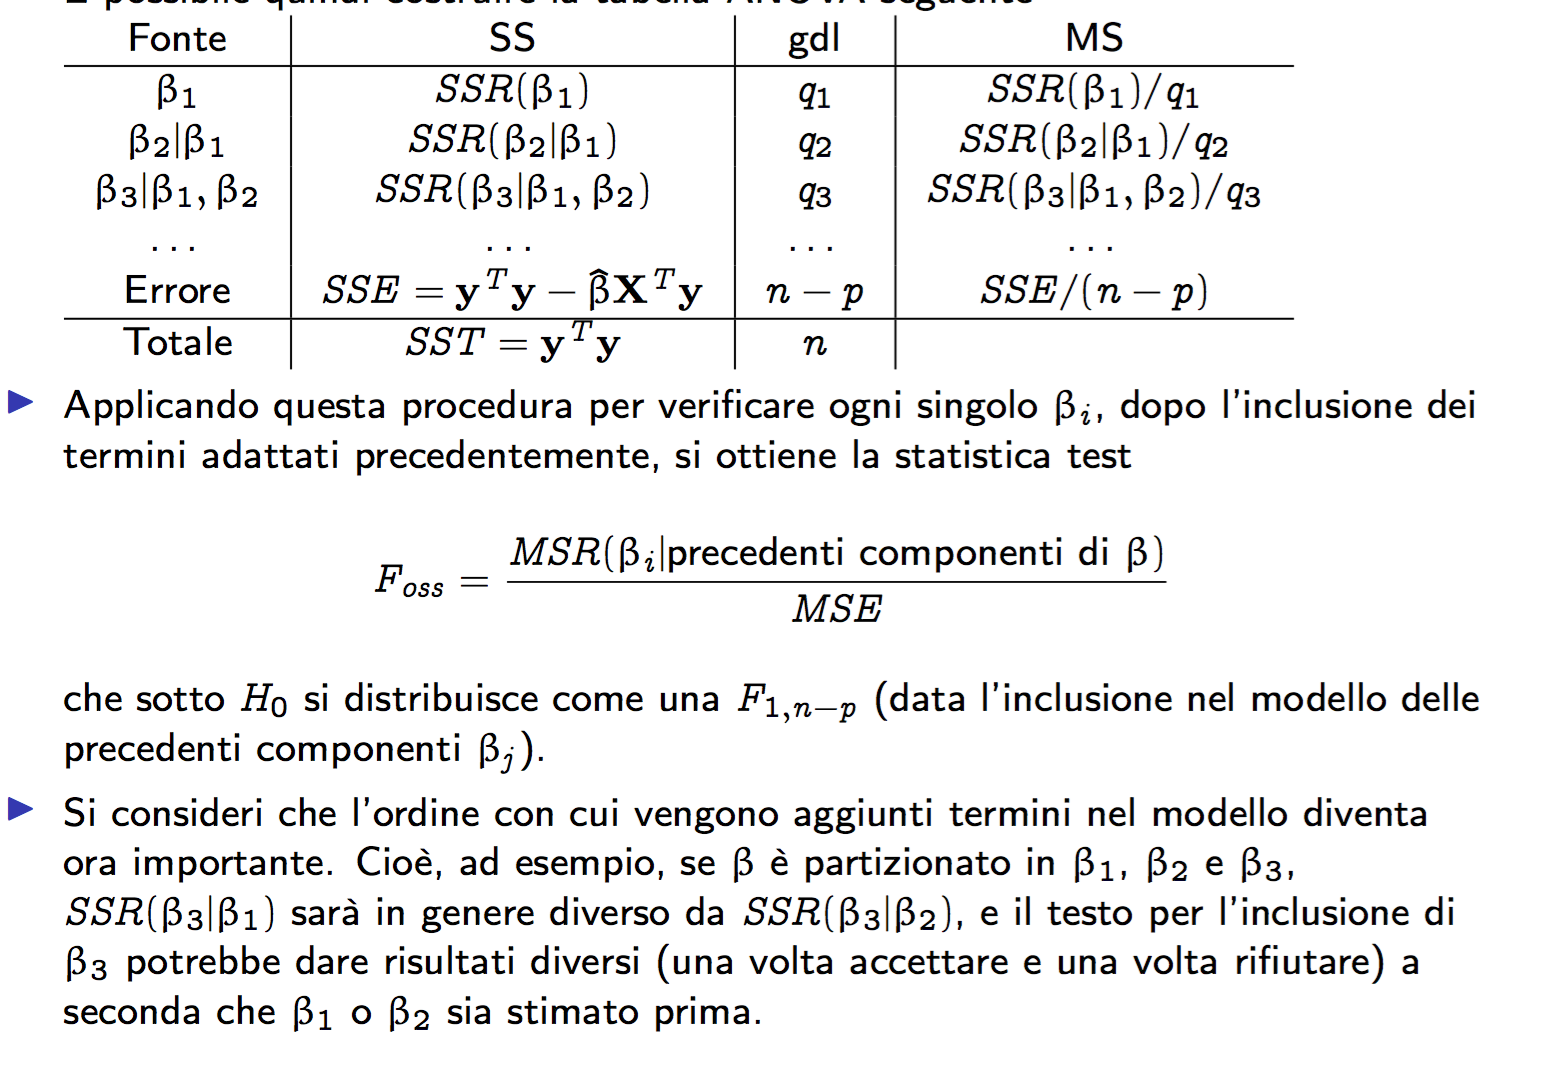
\includegraphics[width=.7\textwidth]{./notes/immagini/l10-fig3.png}
\end{figure}

\begin{figure}[htbp]
	\centering
	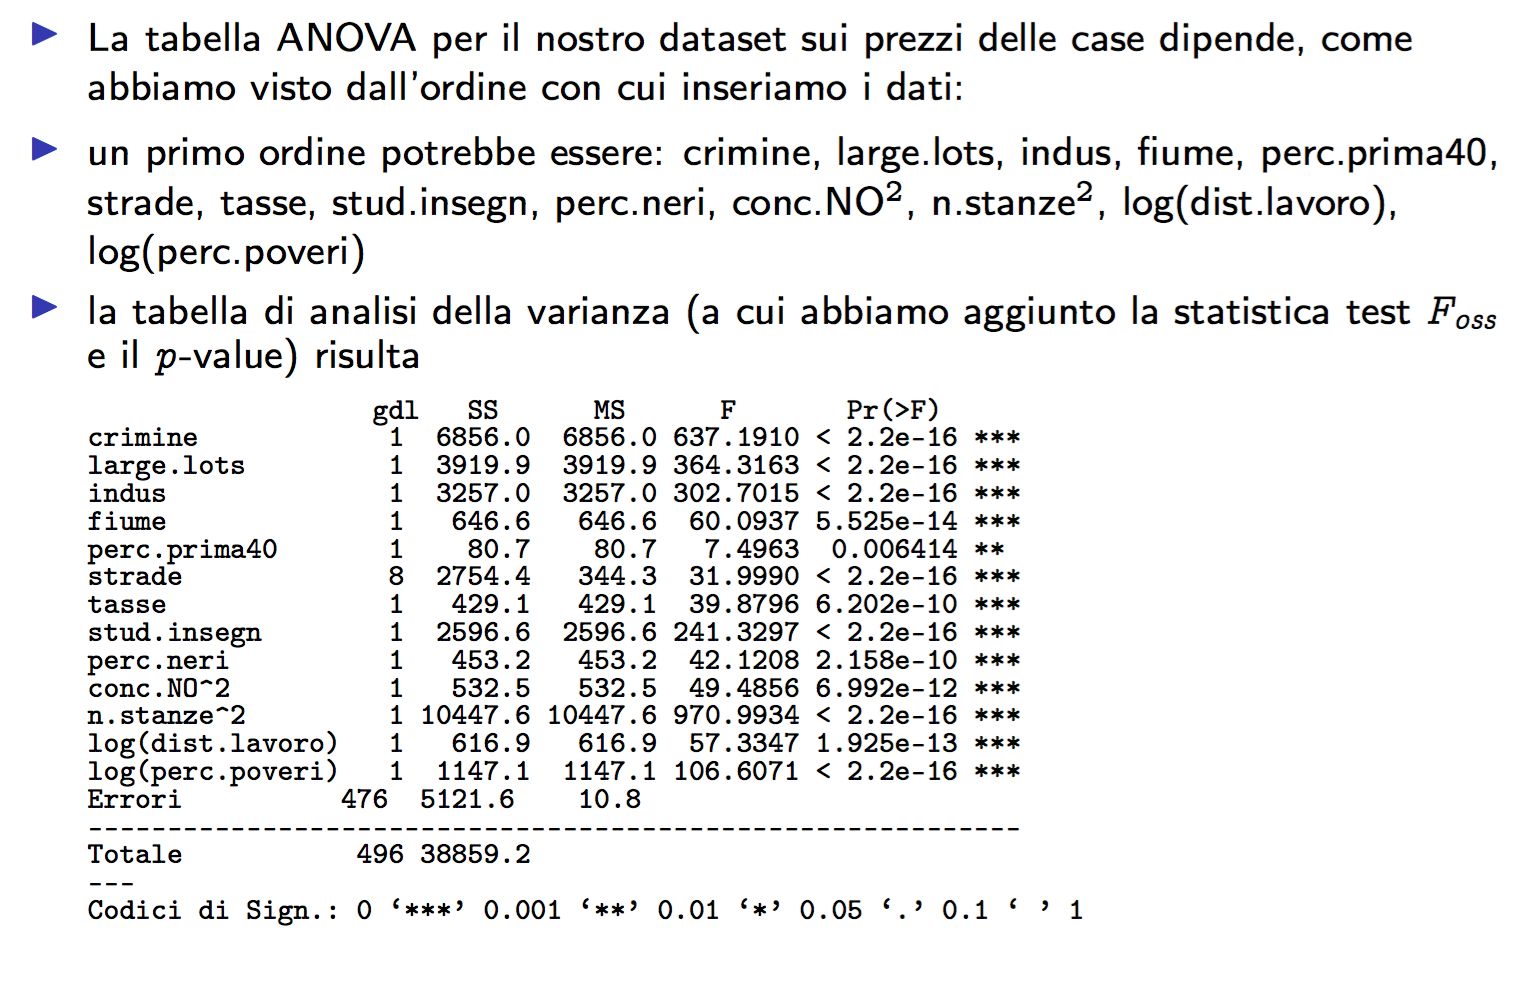
\includegraphics[width=.7\textwidth]{./notes/immagini/l10-fig4.png}
\end{figure}




